\documentclass[11pt]{beamer}
\usepackage[utf8]{inputenc}
\usepackage[T1]{fontenc}
%\usepackage{natbib}
\usetheme{Pittsburgh}
\usepackage{verbatim} 
\usepackage[english]{babel}
\usepackage{epstopdf}
\usepackage{minted}

\definecolor{mygreen}{rgb}{0,0.6,0}
\definecolor{mygray}{rgb}{0.5,0.5,0.5}
\definecolor{mymauve}{rgb}{0.58,0,0.82}
\definecolor{mygray2}{rgb}{0.95,0.95,0.95}

\usepackage{multicol}%\columnseprule  0.4pt\raggedcolumns
%\titlegraphic{%\vspace*{1cm}
%	\includegraphics[width=2.5cm]{logo_udelar}
	%\hspace*{1cm}~%
%		\includegraphics[width=3.5cm]{logo_FCEA.png}
%}
\setbeamertemplate{navigation symbols}{}
\setbeamertemplate{footline}[frame number]
\AtBeginSection{ 
	\begin{frame}
		\frametitle{Index}
			\tableofcontents[currentsection]
	\end{frame}
}
\begin{document}
	\title{Modelos dinámicos y computacionales en Economía}
	\subtitle{Redes y grafos en R}
	%\logo{}
	\institute{Licenciatura en Economía, FCEA, UDELAR}
	\date{3 de octubre de 2024}

	%\subject{}
	%\setbeamercovered{transparent}
	%\setbeamertemplate{navigation symbols}{}
	\frame[plain]{
	\begin{figure}
	\centering
	%
\includegraphics[width=0.7\linewidth]{figuras/netlogo-title-wide-60}
 	
\includegraphics[width=0.2\linewidth]{plots01/Rlogo.eps}

	%		\caption{}
	\label{fig:netlogo-title-wide-60}
\end{figure}	
		\vspace{-1cm}
\maketitle
}
%\setbeamertemplate{background}{\includegraphics[width=2 cm]{logo_FCEA.png}}

\begin{frame}
\frametitle{Contenido de la clase:}
\begin{itemize}
\item Repaso de conceptos
\item (Algunos) tipos de grafos
\item Ejemplo: construcción de un grafo
\item Medidas de centralidad
\item Visualización
%\item Ejemplo: Twitter
\item Redes dinámicas
\end{itemize}
\end{frame}

\begin{frame}{Introducción}
Algunos conceptos importantes:
\begin{itemize}
    \item Nodos, vértices o entidades
\item Aristas, vínculos o relaciones
\item  Análisis de redes, minería de grafos
\item Predicción de enlaces, detección de comunidades/grupos, resolución de entidades, sistema de recomendación, modelado de propagación de información
\end{itemize}
Pasos a seguir:
\begin{enumerate}
\item Construcción del grafo
\item  Medidas de centralidad
\item  Visualización de gráficos
\item Agrupación y detección de comunidades
\end{enumerate}
\end{frame}
%#################

\begin{frame}[fragile]
\frametitle{Análisis de redes sociales} 
Construcción del grafo: ejemplo

\begin{minted}[bgcolor=mygray2,fontsize=\scriptsize]{r}
library(igraph)
g1 <- graph( edges=c(1,2, 2,3, 3,1), n=3, directed=F ) 
# an undirected graph with 3 edges
plot(g1) # A simple plot 
class(g1)
[1] "igraph"
g1

# now with 10 vertices, and directed by default
g2 <- graph( edges=c(1,2, 2,3, 3,1), n=10 ) 
plot(g2)   
g2

g3 <- graph( c("John", "Jim", "Jim", "Jill", "Jill", "John")) # named vertices
# When the edge list has vertex names, the number of nodes is not needed
plot(g3)

gl <- graph_from_literal(a-b-c-d-e-f, a-g-h-b, h-e:f:i, j)
plot(gl)
\end{minted}
\end{frame}

\begin{frame}[fragile]
\frametitle{Análisis de redes sociales} 
\framesubtitle{Tipos de grafos}
\begin{minted}[bgcolor=mygray2,fontsize=\scriptsize]{r}
# Empty graph
eg <- make_empty_graph(40)
plot(eg, vertex.size=10, vertex.label=NA)

# Full graph
fg <- make_full_graph(40)
plot(fg, vertex.size=10, vertex.label=NA)

# Star graph 
st <- make_star(40)
plot(st, vertex.size=10, vertex.label=NA) 

# Tree graph
tr <- make_tree(40, children = 3, mode = "undirected")
plot(tr, vertex.size=10, vertex.label=NA) 

# Ring graph
rn <- make_ring(40)
plot(rn, vertex.size=10, vertex.label=NA)

\end{minted}    
\end{frame}


\begin{frame}[fragile]
\frametitle{Análisis de redes sociales} 
\framesubtitle{Tipos de grafos}
\begin{minted}[bgcolor=mygray2,fontsize=\scriptsize]{r}
# Erdos-Renyi random graph 
# ('n' is number of nodes, 'm' is the number of edges)
er <- sample_gnm(n=100, m=40) 
plot(er, vertex.size=6, vertex.label=NA)  

# Watts-Strogatz small-world graph
sw <- sample_smallworld(dim=2, size=10, nei=1, p=0.1)
plot(sw, vertex.size=6, vertex.label=NA, layout=layout_in_circle)
 
# Barabasi-Albert preferential attachment model for scale-free graphs
 ba <-  sample_pa(n=100, power=1, m=1,  directed=F)
 plot(ba, vertex.size=6, vertex.label=NA)
 
#igraph can also give you some notable historical graphs. For instance:
 zach <- graph("Zachary") # the Zachary carate club
 plot(zach, vertex.size=10, vertex.label=NA)
\end{minted}    
\end{frame}



%#################

\begin{frame}[fragile]
\frametitle{Análisis de redes sociales} 
Construcción del grafo: ejemplo
\begin{itemize}
    \item  $Tom$, $Ben$, $Bob$ y $Mary$ son amigos de $John$.
\item $Alice$ y $Wendy$ son amigas de $Mary$.
\item $Wendy$ es amiga de $David$.
\end{itemize}
\begin{minted}[bgcolor=mygray2,fontsize=\scriptsize]{r}
library(igraph)
# nodos (entidades)
nodes <- data.frame(
name = c("Tom","Ben","Bob","John","Mary","Alice","Wendy","David"),
gender = c("M", "M", "M", "M", "F", "F", "F", "M"),
age =c( 16, 30, 42, 29, 26, 32, 18, 22)
)
# vínculos (relaciones)
edges <- data.frame(
from = c("Tom", "Ben", "Bob", "Mary", "Alice", "Wendy", "Wendy"),
to = c("John", "John", "John", "John","Mary", "Mary", "David")
)
# generar el grafo
g <- graph.data.frame(edges, directed=F, vertices=nodes)    
\end{minted}
\end{frame}


\begin{frame}[fragile]
\frametitle{Análisis de redes sociales} 
Visualizamos el grafo
\begin{itemize}
    \item Todos los nodos
    \item Diferenciados por alguna característica
\end{itemize}
\begin{multicols}{2}
\begin{minted}[bgcolor=mygray2,fontsize=\tiny]{r}
layout1 <- g %>% layout_nicely() 
g %>% plot(vertex.size = 30, layout = layout1)
\end{minted}
\begin{figure}
    \centering
        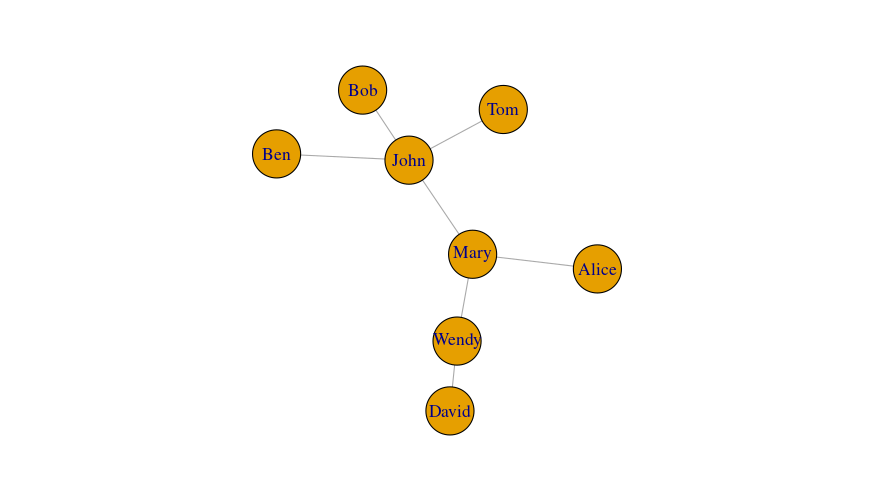
\includegraphics[width=\linewidth]{plots/Captura80.png}
       \end{figure}
\begin{minted}[bgcolor=mygray2,fontsize=\tiny]{r}
colors <- ifelse(V(g)$gender=="M", "green", 
    "yellow")
g %>% plot(vertex.size=30, vertex.color=colors, 
    layout=layout1)
\end{minted}
\begin{figure}
    \centering
        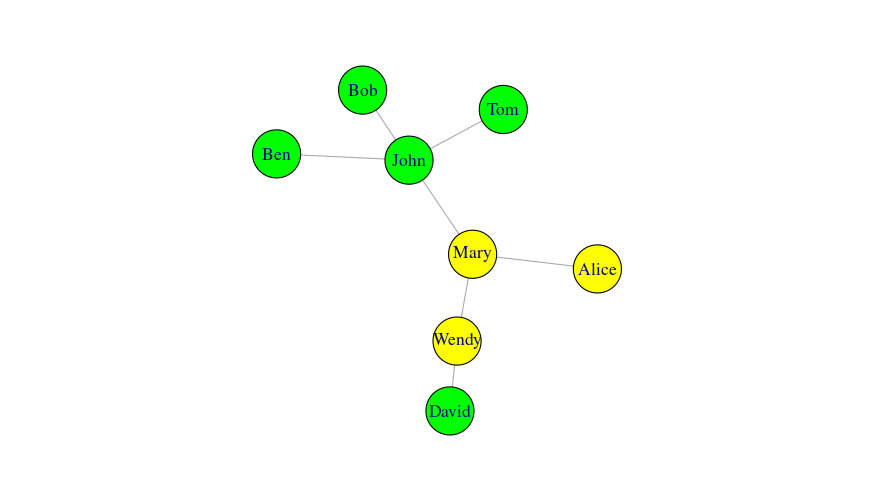
\includegraphics[width=\linewidth]{plots/Captura81.png}
       \end{figure}
\end{multicols}
       
\end{frame}

\begin{frame}[fragile]
\frametitle{Análisis de redes sociales} 
Características de los grafos:
\begin{itemize}
    \item vértices
    \item nodos
    \item vecindad 
\end{itemize}
    \begin{minted}[bgcolor=mygray2,fontsize=\tiny]{r}
## nodes
V(g)
## + 8/8 vertices, named, from 087ce22:
## [1] Tom Ben Bob John Mary Alice Wendy David

## edges
E(g)
## + 7/7 edges from 087ce22 (vertex names):
## [1] Tom --John Ben --John Bob --John John --Mary
## [5] Mary --Alice Mary --Wendy Wendy--David

## immediate neighbors (friends) of John
friends <- ego(g,order=1,nodes="John",mindist=1)[[1]] %>% print()
## + 4/8 vertices, named, from 087ce22:
## [1] Tom Ben Bob Mary

## female friends of John
friends[friends$gender == "F"]
## + 1/8 vertex, named, from 087ce22:
## [1] Mary        
    \end{minted}
\end{frame}

\begin{frame}[fragile]
\frametitle{Análisis de redes sociales} 
Medidas de centralidad
\begin{itemize}   
\item Grado (\textit{degree}): el número de aristas adyacentes; grado y
grado superior para grafos dirigidos
\item Cercanía (\textit{closeness}): el inverso de la longitud promedio de las rutas más cortas hacia/desde todos los demás nodos.
\item Intermediación (\textit{betweenness}): el número de caminos más cortos que atraviesan un nodo.
\end{itemize}
    \begin{minted}[bgcolor=mygray2,fontsize=\tiny]{r}
degree <- g %>% degree() %>% print()
## Tom Ben Bob John Mary Alice Wendy David
##   1   1   1    4    3     1     2     1

closeness <- g %>% closeness() %>% round(2) %>% print()
##  Tom  Ben  Bob John Mary Alice Wendy David
## 0.06 0.06 0.06 0.09 0.09  0.06  0.07  0.05

betweenness <- g %>% betweenness() %>% print()
##Tom Ben Bob John Mary Alice Wendy David
##  0   0   0   15   14    0      6     0     
    \end{minted}
\end{frame}

\begin{frame}[fragile]
 \frametitle{Análisis de redes sociales} 
Visualización de redes estáticas
 \begin{itemize}
       \item Rápido en la representación de gráficos grandes
\item Para gráficos muy grandes, la forma más eficiente es guardar el resultado de la visualización en un archivo, en lugar de hacerlo directamente en la pantalla.
\item Guardar el gráfico de la red en archivos: pdf(), bmp(), jpeg(),
png(), tiff()
   \end{itemize} 
    \begin{minted}[bgcolor=mygray2,fontsize=\scriptsize]{r}
## graficar directamente en la pantalla
plot(g)
## para gráficos grandes, guardar en PDF
pdf("mygraph.pdf")
plot(g)
dev.off() 
    \end{minted}
\end{frame}


\begin{comment}
    
\begin{frame}[fragile]
 \frametitle{Análisis de redes sociales} 
Ejemplo con datos de Twitter, en cuentas verificadas:
\begin{minted}[bgcolor=mygray2,fontsize=\scriptsize]{r}
sli <- search_tweets("#tourism OR #travel OR #hospitality 
    AND filter:images AND filter:verified", lang= "en", n=1000)
# graficamos
ts_plot(sli, by = "hours")
sli %>%
  dplyr::group_by(is_retweet) %>%
  ts_plot("hours")
    \end{minted}
  \begin{figure}
    \centering
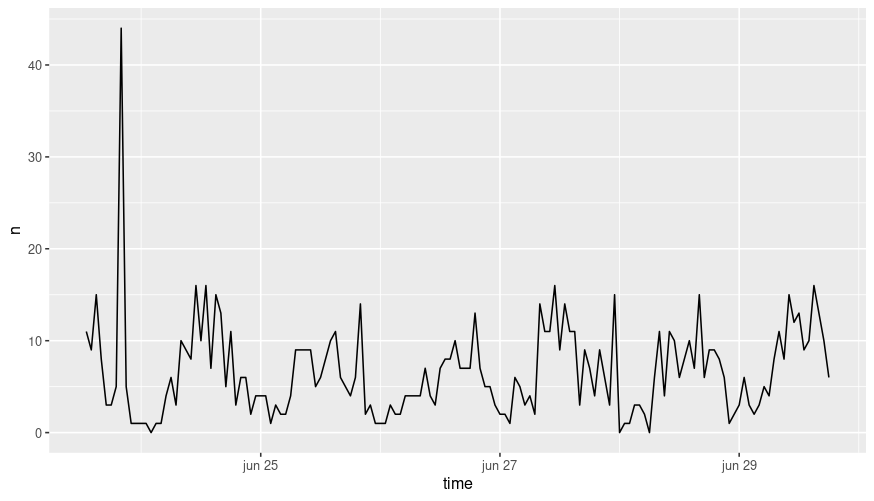
\includegraphics[width=0.45\linewidth]{plots/Captura82.png}
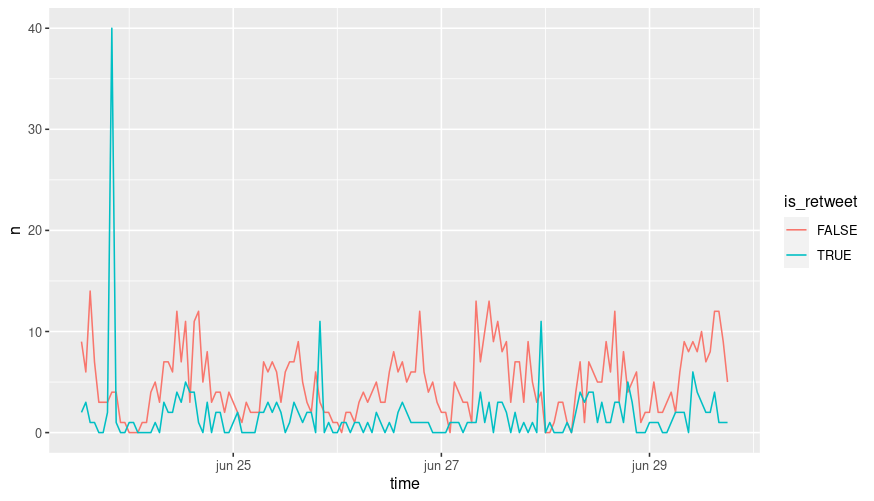
\includegraphics[width=0.45\linewidth]{plots/Captura83.png}        
       \end{figure} 
\end{frame}

\begin{frame}[fragile]
 \frametitle{Análisis de redes sociales} 
Ejemplo con datos de Twitter, en cuentas verificadas:
\begin{itemize}
    \item wordcloud
\end{itemize}
  \begin{figure}
    \centering

\includegraphics[width=0.55\linewidth]{plots/Captura85.png}
       \end{figure} 
\end{frame}

\begin{frame}[fragile]
 \frametitle{Análisis de redes sociales} 
Ejemplo con datos de Twitter, en cuentas verificadas:
\begin{minted}[bgcolor=mygray2,fontsize=\tiny]{r}
# seleccionamos algunas columnas
netdf=sli%>%dplyr::select(.,screen_name,retweet_screen_name,is_retweet)
# sólo nos quedamos con aquellos con retweet
netdfr=netdf%>%filter(is_retweet)%>%select(-is_retweet) 
netdfp=netdf%>%filter(!is_retweet)%>%pull(screen_name)
net_graph=graph_from_data_frame(netdfr)#+netdfp
E(net_graph)$weight=rep(1,ecount(net_graph))
net_graph_s <- igraph::simplify( net_graph, remove.multiple = T, remove.loops = F, 
                                 edge.attr.comb=c(weight="sum"))
net_graph_s
# plot, con diferencias en los tamaños de los nodos según su degree
plot(net_graph_s,vertex.color="gold", vertex.size=log(igraph::degree(net_graph_s))*3+1, 
     vertex.frame.color="gray", vertex.label.color="black", 
     vertex.label.cex=log(igraph::degree(net_graph_s))*0.6+0.1, vertex.label.dist=2, 
     edge.curved=0.5,edge.arrow.size=.2)
    \end{minted}
\end{frame}


\begin{frame}[fragile]
 \frametitle{Análisis de redes sociales} 
Ejemplo con datos de Twitter, en cuentas verificadas:
\begin{figure}
    \centering
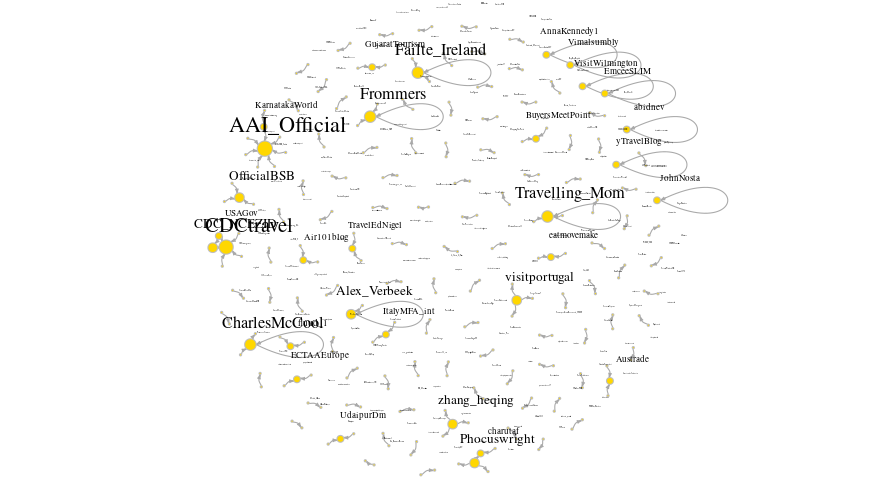
\includegraphics[width=\linewidth]{plots/Captura84.png}        
       \end{figure} 
\end{frame}
\end{comment}

\begin{comment}
\begin{frame}[fragile]
 \frametitle{Análisis de redes sociales} 
Red de seguidores y retweets
\begin{minted}[bgcolor=mygray2,fontsize=\tiny]{r}# seleccionamos algunas columnas
library(rtweet)
library(tidyverse)

user.seed="fcea_udelar"
user.following=get_friends(user.seed,n=500,retryonratelimit = TRUE)
nrow(user.following)
user.following%>%head(5)
info.following=lookup_users(user.following$user_id)
info.following
##criterio: description, verified (blue check mark), location
info.following%>%select(geo_coords,country,country_code,location,description)%>%lat_lng()
## filter based on description
candidates=info.following%>%filter(description%>%
                                     str_detect("udelar|UDELAR|UdelaR|Universidad"),
                                   description%>%
                                     str_detect("FCEA|Econom|Económ"))%>%
  select(user_id,screen_name,name,friends_count,description)
candidates%>%head
candidates
    \end{minted}
\end{frame}

\begin{frame}[fragile]
 \frametitle{Análisis de redes sociales} 
Red de seguidores: \texttt{candidates}
\begin{minted}[bgcolor=mygray2,fontsize=\tiny]{r}# seleccionamos algunas columnas
# A tibble: 15 × 5
   user_id             screen_name     name                             friends_count description                   
   <chr>               <chr>           <chr>                                    <int> <chr>                         
 1 1262138678484307969 HWillebald      Henry Willebald                             95 I am economist (UdelaR) and P…
 2 1243983276542435328 IestaUdelar     Instituto de Estadística (IESTA)           217 Instituto de Investigación de…
 3 1372905366686732288 UACYGdeFCEA     UA Costos y Control de Gestión              29 Twitter oficial de la Unidad …
 4 298280745           EmaZel          Ema Zelikovitch                           1743 Comunicadora @FCEA_UdelaR y @…
 5 4518581             gbudino         Gabriel Budiño                            1000 Uruguayo. Contador Público (U…
 6 1324932745          MartinVallcorba Martin Vallcorba                           973 Economista (UdelaR, Universid…
 7 620563766           BrunoAgustoni   Bruno Agustoni                             542 Economista | MA in Public Pol…
 8 1410541032          joatotes        Joaquín Toledo Tesoro                     1733 Economista daltónico • Docent…
 9 1529107477          elenasivori     Elena Sívori ����                            468 Bisnieta de india e inmigrant…
10 892037303086047232  deFCEA          Departamento de Economía FCEA              150 Twitter oficial del Departame…
11 755819601947160576  dECON_UdelaR    dECON                                      136 Departamento de Economía, FCS…
12 488649030           cguccee         CGU Economía                               132 FCEA-UdelaR Gremio libre e in…
13 1001779501          BibliotecaFcea  BIBLIOTECA FCEA                            521 Biblioteca de la Facultad de …
14 946708764           gatefceaudelar  GATE FCEA UdelaR                           105 El GATE es un equipo multidis…
15 287975317           RodrigoArim1    Rodrigo Arim                              1770 Rector de la Universidad de l…
    \end{minted}
\end{frame}

\begin{frame}[fragile]
 \frametitle{Análisis de redes sociales} 
Red de vínculos entre seguidores
\begin{enumerate}
    \item Generar la red de seguidores de \texttt{``fcea\_udelar''}
\end{enumerate}
\begin{minted}[bgcolor=mygray2,fontsize=\tiny]{r} 
user.seed= "fcea_udelar"
user.following=get_friends(user.seed,retryonratelimit = TRUE)
userid=c(user.seed,user.following$user_id)
info.following=lookup_users(userid)
user.df=info.following%>%
  filter(description%>% str_detect("UDELAR|UdelaR|FCEA|Econ|ccee"),
         friends_count > 0) %>%
  select(user_id,screen_name,name,friends_count,description)
acc.id=user.df$user_id # qualified id
nyc.id=user.seed # already scrapped the friends
can.id=acc.id[!acc.id%in%nyc.id] # to be scrapped
rej.id=userid[!info.following$user_id%in%acc.id] # non-qualified
edge.list=user.following%>%filter(user_id%in%acc.id) # network
info.id=userid # already request user info
   \end{minted}
\end{frame}

\begin{frame}[fragile]
 \frametitle{Análisis de redes sociales} 
Red de vínculos entre seguidores
\begin{enumerate}  \setcounter{enumi}{1}
    \item Generar la red de seguidores de los seguidores de \texttt{``fcea\_udelar''}
\end{enumerate}
\begin{minted}[bgcolor=mygray2,fontsize=\tiny]{r} 
while((length(nyc.id)<100)){
  # pick the first user in the acc.id
  user.following=get_friends(can.id,n=1000,retryonratelimit = TRUE)
  userid=user.following$user_id
  useridx=userid[!userid%in%info.id] # new userid
  info.following=lookup_users(useridx)
  user.dfx=info.following%>%filter(description%>%
           str_detect(regex("UDELAR|UdelaR|FCEA|Econ|ccee",ignore_case = T))
  )%>%
    select(user_id,screen_name,name,friends_count,description)
  nyc.id=c(nyc.id,can.id)%>%unique() #already scrapped and in the list
  if(nrow(user.dfx)==0){break}
  user.df=rbind(user.df,user.dfx) #merge user info df
  can.id=user.dfx$user_id #to be scrapped
  rej.idx=useridx[!useridx%in%can.id] #not qualified
  rej.id=c(rej.id,rej.idx)%>%unique()
  acc.id=c(acc.id,can.id)%>%unique()
  info.id=c(info.id,useridx)%>%unique()
  edge.listx=user.following%>%filter(user_id%in%acc.id) #add edgelist
  edge.list=rbind(edge.list,edge.listx)
}
edge.list%>%head(5)
user.df%>%head(5)
    \end{minted}
\end{frame}

\begin{frame}[fragile]
 \frametitle{Análisis de redes sociales} 
Red de vínculos entre seguidores
\begin{enumerate}  \setcounter{enumi}{2}
    \item Generar el grafo a partir de los nodos y links que se encuentran en \texttt{edge\_list}
\end{enumerate}
\begin{minted}[bgcolor=mygray2,fontsize=\tiny]{r} 
net=graph_from_data_frame(edge.list)
netsim=igraph::simplify(net, remove.multiple = T, remove.loops = T)
V(netsim)$id=V(netsim)$name

user.df=user.df %>%
  unique()%>%
  arrange(match(user_id, V(netsim)$id))
user.name=user.df%>%
  pull(name)
V(netsim)$name=user.name
V(netsim)$degree=user.df$friends_count
set.seed(123)
plot(netsim,vertex.name=V(netsim)$user.name,vertex.color="gold",
    vertex.size=log(V(netsim)$degree)*.8+0.01, 
    vertex.frame.color="gray", vertex.label.color="black",
    vertex.label.cex=0.5, vertex.label.dist=1, 
    edge.curved=0.5,edge.arrow.size=.2,
    vertex.label.cex=.5,vertex.label=user.name)
\end{minted}
\end{frame}    
\end{comment}


\begin{frame}[fragile]
\frametitle{Redes dinámicas}
\framesubtitle{Ejemplo: familias renacentistas}
    \begin{minted}[bgcolor=mygray2,fontsize=\tiny]{r} 
library('network')
library('igraph')
data(flo)
nflo=graph_from_adjacency_matrix(flo,mode='undirected',add.colnames=T)
summary(nflo)
V(nflo)$name=row.names(flo)
library('igraph')
plot(nflo)
results=cbind(igraph::degree(nflo),igraph::betweenness(nflo),igraph::closeness(nflo),
              round(igraph::eigen_centrality(nflo)$vector,8))
row.names(results)=colnames(flo)
colnames(results)=c('degree','betweenness','closeness','eigen')     
    \end{minted}
 
%    \vspace{-0.5cm}

\begin{figure}
    \centering
    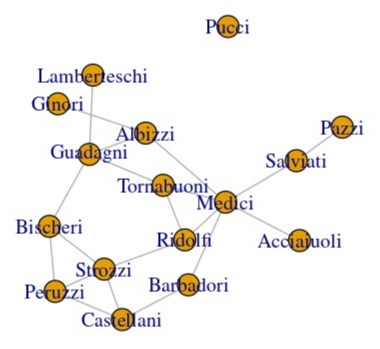
\includegraphics[width=0.40\linewidth]{plots/florentine.png}
 %   \caption{Caption}
    \label{fig:my_label}
\end{figure}    
\end{frame}

\begin{frame}[fragile]
\frametitle{Redes dinámicas}
\framesubtitle{Ejemplo: familias renacentistas - dinámica de formación de vínculos}
    \begin{minted}[bgcolor=mygray2,fontsize=\tiny]{r} 
library('ndtv')
data(short.stergm.sim)
head(as.data.frame(short.stergm.sim))
render.d3movie(short.stergm.sim,displaylabels=TRUE,output.mode = "htmlWidget") 

library('tsna')
plot(tEdgeFormation(short.stergm.sim, time.interval = 1),ylab="edge_formation")
    \end{minted}
 
%    \vspace{-0.5cm}

\begin{figure}
    \centering
    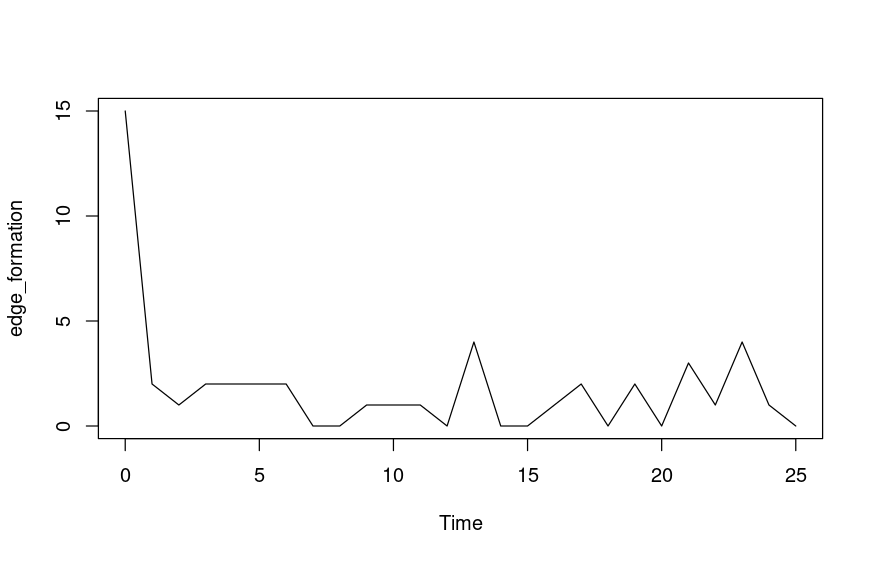
\includegraphics[width=0.55\linewidth]{plots/tsna_1.png}
 %   \caption{Caption}
    \label{fig:my_label}
\end{figure}    
\end{frame}

\begin{frame}[fragile]
\frametitle{Redes dinámicas}
\framesubtitle{Ejemplo: familias renacentistas - betweenness y tamaño del componente mayor}
\begin{columns}
\begin{column}{0.4\linewidth}
\begin{minted}[bgcolor=mygray2,fontsize=\tiny]{r} 
dynamicBetweenness <- tSnaStats(
  short.stergm.sim,
  snafun = "centralization",
  start = 1,
  end = 25,
  time.interval = 1,
  aggregate.dur = 0, # 'seasonality'
  FUN = "betweenness"
)
plot(dynamicBetweenness)

dynamicComponents <- tSnaStats(
  short.stergm.sim,
  snafun = "components",
  start = 1,
  end = 25,
  time.interval = 1,
  aggregate.dur = 0, 
)
plot(dynamicComponents)
    \end{minted}
    \end{column}
 
\begin{column}{0.4\linewidth}
    \begin{figure}
    \centering
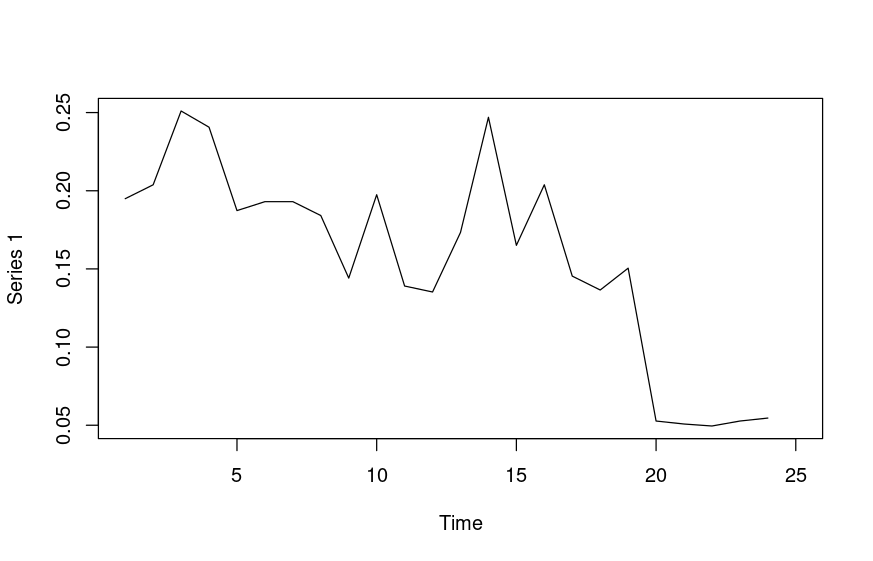
\includegraphics[width=0.9\linewidth]{plots/tsna_2.png}
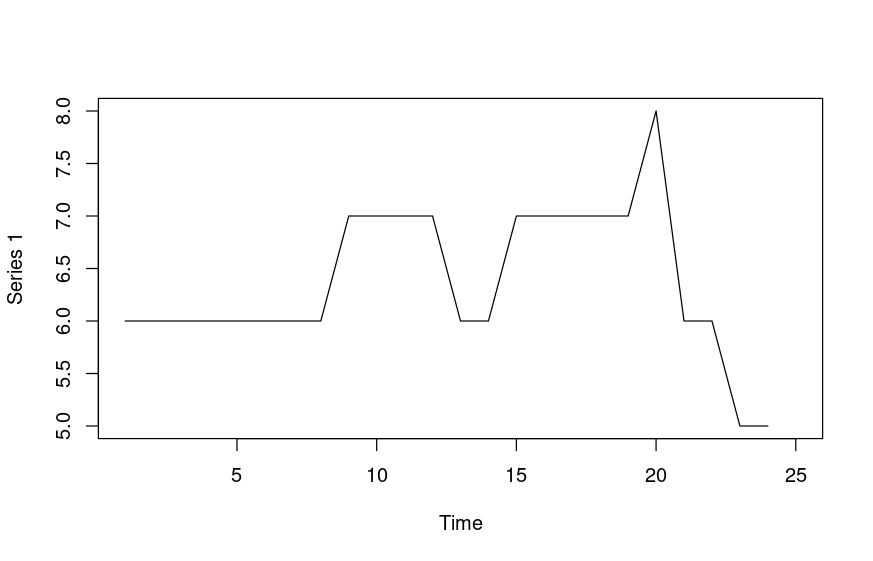
\includegraphics[width=0.9\linewidth]{plots/tsna_3.png}

 %   \caption{Caption}
    \label{fig:my_label}
\end{figure}    
\end{column}
\end{columns}

\end{frame}

\begin{frame}[fragile]
\frametitle{Redes dinámicas}
\framesubtitle{Ejemplo: familias renacentistas - densidad y transitividad}
\begin{columns}
\begin{column}{0.4\linewidth}
\begin{minted}[bgcolor=mygray2,fontsize=\tiny]{r} 
dynamicDen <- tSnaStats(
  short.stergm.sim,
  snafun = "gden",
  start = 1,
  end = 25,
  time.interval = 1,
  aggregate.dur = 0, 
)
plot(dynamicDen)

dynamicTr <- tSnaStats(
  short.stergm.sim,
  snafun = "gtrans",
  start = 1,
  end = 25,
  time.interval = 1,
  aggregate.dur = 0, 
)
plot(dynamicTr)

    \end{minted}
    \end{column}
 
\begin{column}{0.4\linewidth}
    \begin{figure}
    \centering
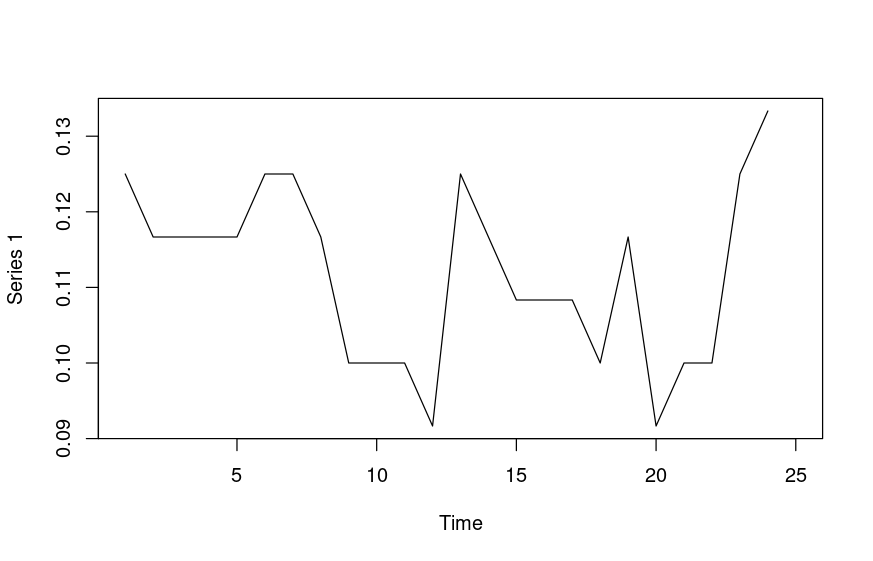
\includegraphics[width=0.9\linewidth]{plots/tsna_4.png}
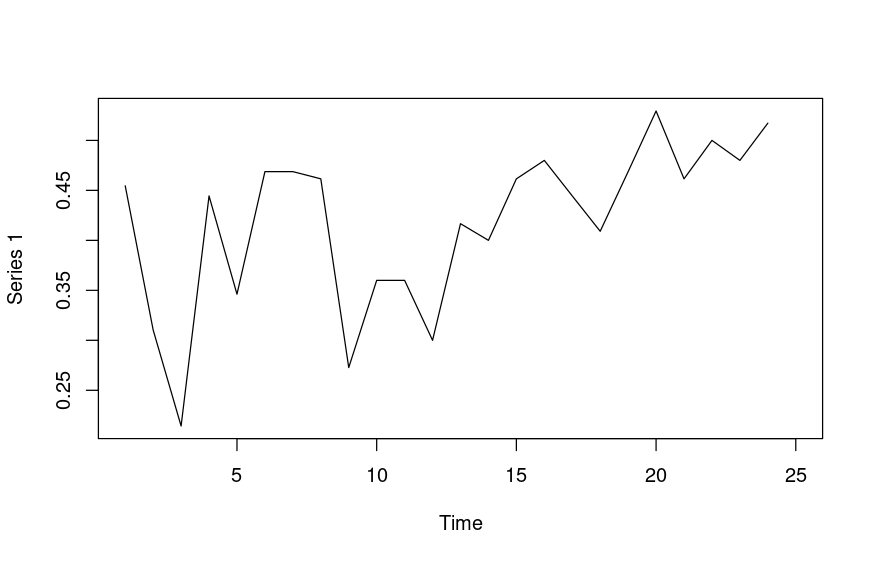
\includegraphics[width=0.9\linewidth]{plots/tsna_5.png}

 %   \caption{Caption}
    \label{fig:my_label}
\end{figure}    
\end{column}
\end{columns}
\end{frame}

\begin{frame}[fragile]
\frametitle{Redes dinámicas}
\framesubtitle{Ejemplo: familias renacentistas - conexiones a través de la red temporal}
\begin{columns}
\begin{column}{0.4\linewidth}
\begin{minted}[bgcolor=mygray2,fontsize=\tiny]{r} 
plot(tReach(short.stergm.sim,
direction="fwd"))

set.seed(110)
RidolfiFwdPath <- tPath(
  short.stergm.sim,
  v = 13,
  direction = "fwd"
)
plotPaths(
  short.stergm.sim,
  RidolfiFwdPath,
  displaylabels = T,
  vertex.col = "green",
  edge.label.col="blue"
)

    \end{minted}
    \end{column}
 
\begin{column}{0.4\linewidth}
    \begin{figure}
    \centering
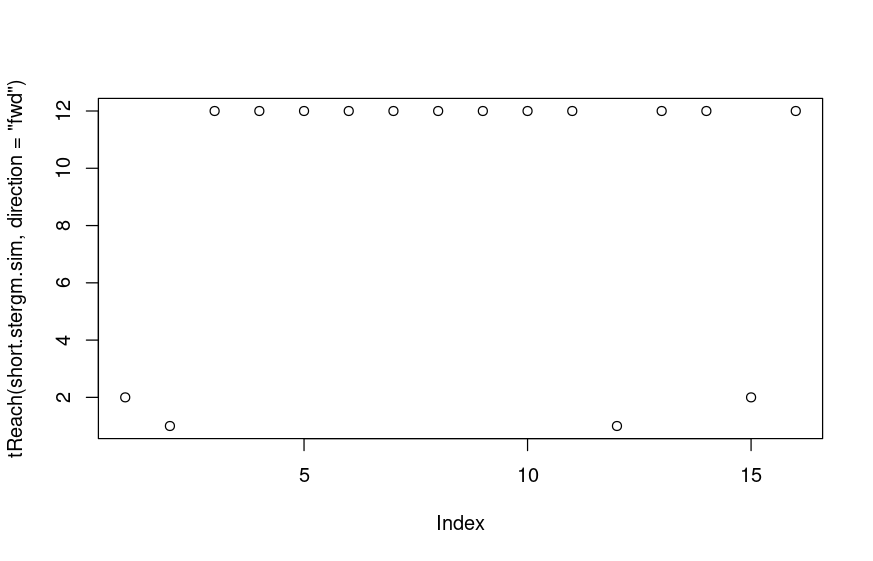
\includegraphics[width=0.9\linewidth]{plots/tsna_6.png}
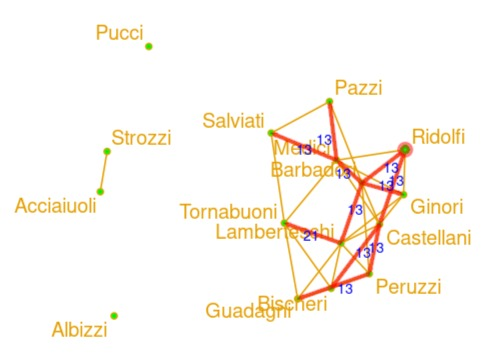
\includegraphics[width=0.9\linewidth]{plots/tsna_7.png}

 %   \caption{Caption}
    \label{fig:my_label}
\end{figure}    
\end{column}
\end{columns}
\end{frame}


\end{document}
